%\section {Results}
\label{results}

%\subsection {Analysis} 
%Since $H_{1}$ concerns the mean count of xyz for each word, a one-tailed Student's Independent \textit{t}-test will be used here to determine whether the mean count of xyz for nouns are statistically significantly greater than those for adjectivs.  The threshold for significance adopted here is $0.01$.  

%\subsection{Total RMSE (Error Over All Imitation Types)}
Figure \ref{fig:overall} shows the overall error for each variation of the genetic algorithm. The best algorithm was algorithm 1 with an RMSE of $184.89$ while the worst, algorithm 8, had an RMSE of $188.82$. %Since the genetic alignment algorithms are all deterministic in nature, these errors are always the same. Subsequently, their standard deviation is 0 and their average is what they are. This makes them statistically significantly different. Thus, with $p < 0.00...01$, algorithm 1 is better than all other algorithms thus far demonstrated.

\begin{figure}[center]
	\centering
	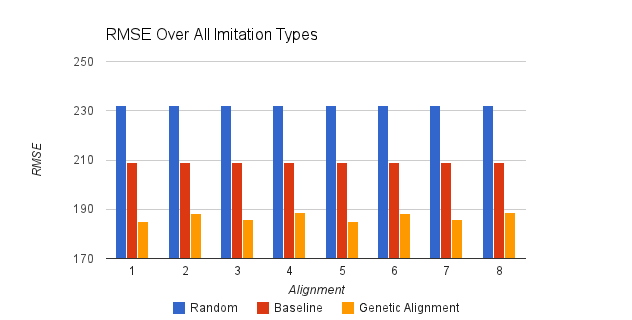
\includegraphics[width=16cm]{images/chart9.png}
	\caption{Note that genetic alignment outperformed baseline in all cases.}
	\label{fig:overall}
\end{figure}

%\subsection{Error By Imitation Class}
To demonstrate the preferences inherent in each genetic alignment algorithm, we compute the RMSE for each with respect to each citation type. They each exhibited behaviors that were interesting. For example, genetic alignment 2 was best for imitations of type 2. The best genetic algorithm for each class is given in table \ref{tab:best-for-each}.

\begin{table}[center]
	\centering
	\begin{center}
		\begin{tabular}{|l|c|c|} \hline
			\textbf{Imitation Type}	& \textbf{Best Algorithm}	&	\textbf{Error (RMSE)}	\\ \hline \hline
			1						& 1							&	147.08					\\ \hline
			2						& 2							&	272.56					\\ \hline
			3						& 1							&	161.01					\\ \hline
			4						& 1							&	271.10					\\ \hline
			5						& 1							&	183.64					\\ \hline
			6						& 1							&	182.76					\\ \hline
			7						& 1							&	73.94					\\ \hline
		\end{tabular}
	\end{center}
	\caption{Algorithm 1 has the best RMSE for $6/7$ of the imitation types.}
	\label{tab:best-for-each}
\end{table}

Interestingly, algorithm 1 is often the best algorithm. Subsequently, this is also true for the RMSE over all imitation types. Algorithm 1 combined wih BP-MLP ends up being the best high-order combinational model. However, in when simple linear regression is used, algorithm 1 ends up being the worst model.